%%%%%%%%%%%%%%%%%%%%%%%%%%%%%%%%%%%%%%%%%%%%%%%%%%%%%%%%%%%%%%%%%%%%%%%%%%%%%%%
% M.Sc. Libre Software URJC 2013
%
% Master Thesis
% Esther Parrilla-Endrino (eparrillae@gmail.com)
%
%%%%%%%%%%%%%%%%%%%%%%%%%%%%%%%%%%%%%%%%%%%%%%%%%%%%%%%%%%%%%%%%%%%%%%%%%%%%%%%

\documentclass[a4paper,12pt]{book} 
\usepackage[utf8]{inputenc}
\usepackage[english]{babel}
\usepackage{url}
\usepackage[colorlinks=true,linkcolor=black,urlcolor=black]{hyperref} 
%%%%%%%%%%%%%%%%%%%%%%%%%%%%%%%%%%%%%%%%%%%%%%%%%%%%%%%%%%%%%%%%
%% ccBeamer 0.1, 2007-07-02                                   %%
%% Written by Sebastian Pipping <webmaster@hartwork.org>      %%
%% ---------------------------------------------------------- %%
%% Licensed under Creative Commons Attribution-ShareAlike 3.0 %%
%% http://creativecommons.org/licenses/by-sa/3.0/             %%
%%%%%%%%%%%%%%%%%%%%%%%%%%%%%%%%%%%%%%%%%%%%%%%%%%%%%%%%%%%%%%%%


%% Images
\newcommand{\CcImageBy}[1]{%
	
\includegraphics[scale=#1]{creative_commons/cc_by_30.pdf}%
}
\newcommand{\CcImageCc}[1]{%
	
\includegraphics[scale=#1]{creative_commons/cc_cc_30.pdf}%
}
\newcommand{\CcImageDevNations}[1]{%
	
\includegraphics[scale=#1]{creative_commons/cc_dev_nations_30.pdf}%
}
\newcommand{\CcImageNc}[1]{%
	
\includegraphics[scale=#1]{creative_commons/cc_nc_30.pdf}%
}
\newcommand{\CcImageNd}[1]{%
	
\includegraphics[scale=#1]{creative_commons/cc_nd_30.pdf}%
}
\newcommand{\CcImagePd}[1]{%
	
\includegraphics[scale=#1]{creative_commons/cc_pd_30.pdf}%
}
\newcommand{\CcImageSa}[1]{%
	
\includegraphics[scale=#1]{creative_commons/cc_sa_30.pdf}%
}
\newcommand{\CcImageSampling}[1]{%
	
\includegraphics[scale=#1]{creative_commons/cc_sampling_30.pdf}%
}
\newcommand{\CcImageSamplingPlus}[1]{%
	
\includegraphics[scale=#1]{creative_commons/cc_sampling_plus_30.pdf}%
}


%% Groups
\newcommand{\CcGroupBy}[1]{% zoom
	\CcImageBy{#1}%
}
\newcommand{\CcGroupByNc}[2]{% zoom, gap
	\CcImageBy{#1}\hspace*{#2}\CcImageNc{#1}%
}
\newcommand{\CcGroupByNcNd}[2]{% zoom, gap
	\CcImageBy{#1}\hspace*{#2}\CcImageNc{#1}\hspace*{#2}\CcImageNd{#1}%
}
\newcommand{\CcGroupByNcSa}[2]{% zoom, gap
	\CcImageBy{#1}\hspace*{#2}\CcImageNc{#1}\hspace*{#2}\CcImageSa{#1}%
}
\newcommand{\CcGroupByNd}[2]{% zoom, gap
	\CcImageBy{#1}\hspace*{#2}\CcImageNd{#1}%
}
\newcommand{\CcGroupBySa}[2]{% zoom, gap
	\CcImageBy{#1}\hspace*{#2}\CcImageSa{#1}%
}
\newcommand{\CcGroupDevNations}[1]{% zoom
	\CcImageDevNations{#1}%
}
\newcommand{\CcGroupNcSampling}[2]{% zoom, gap
	\CcImageNc{#1}\hspace*{#2}\CcImageSampling{#1}%
}
\newcommand{\CcGroupPd}[1]{% zoom
	\CcImagePd{#1}%
}
\newcommand{\CcGroupSampling}[1]{% zoom
	\CcImageSampling{#1}%
}
\newcommand{\CcGroupSamplingPlus}[1]{% zoom
	\CcImageSamplingPlus{#1}%
}


%% Text
\newcommand{\CcLongnameBy}{Attribution}
\newcommand{\CcLongnameByNc}{Attribution-NonCommercial}
\newcommand{\CcLongnameByNcNd}{Attribution-NoDerivs}
\newcommand{\CcLongnameByNcSa}{Attribution-NonCommercial-ShareAlike}
\newcommand{\CcLongnameByNd}{Attribution-NoDerivs}
\newcommand{\CcLongnameBySa}{Attribution-ShareAlike}

\newcommand{\CcNote}[1]{% longname
	This work is licensed under the \textit{Creative Commons #1 3.0 License}.%
}

\usepackage{amssymb}
\usepackage{eurosym}
\usepackage{verbatim}
\usepackage{fancyhdr} 
\usepackage{amsmath}
\usepackage{graphicx}
\usepackage{pdfpages}
\usepackage{float}
\usepackage{caption3} 
\DeclareCaptionOption{parskip}[]{} 
\usepackage[small]{caption}
\usepackage{latexsym}  %% For additional characters
\usepackage{rotating}
\usepackage[table]{xcolor}

\title {Trade-Off Analysis of Open Source Web Mobile App Frameworks: The KuDo Project}
\author{Esther Parrilla-Endrino (eparrillae@gmail.com)\\
 M.Sc. Libre Software URJC}
\date{\today}

\renewcommand{\baselinestretch}{1.5}  

\begin{document}

%%%%%%%%%%%%% First Page %%%%%%%%%%%%%%%%
\begin{titlepage}
\begin{center}
\begin{tabular}[c]{c c}

\includegraphics[scale=0.25]{img/logo.png} &
\begin{tabular}[b]{l}
\Huge
\textsf{UNIVERSIDAD} \\
\Huge
\textsf{REY JUAN CARLOS} \\
\end{tabular}
\\
\end{tabular}

\vspace{3cm}

\Large
Free Libre Open Source Software Master

\vspace{0.4cm}

\large
Academic Year 2012/2013

\vspace{0.4cm}

Master Thesis

\vspace{1cm}

\LARGE
Trade-Off Analysis of Open Source Web Mobile App Frameworks: The KuDo Project

\begin{figure}[H]
    \centering
    
\includegraphics[width=4cm, keepaspectratio]{img/kudologo.png}
 \end{figure}

%\vspace{4cm}

\large
Author: Esther Parrilla-Endrino \\
Tutors: Prof. Gregorio Robles, Prof. Daniel Izquierdo 
\end{center}
\end{titlepage}
%%%%%%%%%%%%%%%%%%%%%%%%%%%%%%%%%%%%%%

\newpage
\thispagestyle{empty}
\vspace{5cm}
\begin{flushright}
\begin{large}
Copyright \copyright 2013 Esther Parrilla-Endrino.\\
Some Rights Reserved.\\
This work is licensed under the\\
Creative Commons Attribution 3.0 License.\\
To view a copy of this license, visit\\
\url{http://creativecommons.org/licenses/by/3.0/}\\
or send a letter to Creative Commons,\\
543 Howard Street, 5th Floor, San Francisco,\\
California, 94105, USA.\\
\end{large}
\end{flushright}

\newpage

\tableofcontents  %% contents index

\renewcommand{\refname}{Bibliography}
\addtolength{\parskip}{\baselineskip}

%%%%%%%%%%%%%%%%%%%%%%%%%%%%%%%%%%%%%%%%%%%%%%%%%%%%%%%%%%%%%%%%%%%%%

\chapter*{Summary}
\label{chap:summary}

In my daily work I play the role of Technical Manager who coordinates the development of both standalone and web solutions for the Aerospace field, therefore I have no possibility of working in projects related to mobile apps implementation which is one of the most interesting activity nowadays.

Beginning this year I have started working on a personal project called 'KuDo', the idea is to setup a start-up focused in the development of web-based applications for educational purposes that can be easily run in mobile devices such as smartphones, tablets etc...

This Master Thesis is the baseline activity I have performed for the KuDo project in order to determine which technical solution could fit better for this purpose from the wide range of web mobile app frameworks existing nowadays.

All paper work done for this Master Thesis is Open Source material licensed under a Creative Commons Attribution 3.0 License\footnote{http://creativecommons.org/licenses/by/3.0/} and the code of the prototypes implemented in the context of this thesis is under MIT License\footnote{http://opensource.org/licenses/MIT}.

All these activities have been developed using GitHub repository and can be downloaded from the following url:

\url{
https://github.com/eparrillae/eparrillae-mswl-thesis.git}

Also the different activities performed in this Master Thesis have been described in my personal blog and can be found under the following tag:

\url{
http://eparrillae.net/wordpress/?tag=mswl-thesis}

I would like to thank my Master Thesis tutors Gregorio Robles\footnote{http://gsyc.urjc.es/grex/} and Daniel Izquierdo\footnote{http://www.linkedin.com/in/dicortazar} for guiding the whole process, always providing good advices and added-value to this work.

Finally I would like to specially thank my colleague Solange Molina Urrutia\footnote{http://www.linkedin.com/in/smolina} who has been a reference for me in this work due to her huge background expertise in mobile app developments.  

%%%%%%%%%%%%%%%%%%%%%%%%%%%%%%%%%%%%%%

\chapter{Overview and Objectives}
\label{chap:overview}

Nowadays mobile devices such as smartphones and tablets have become the preferred tools for communicating with each other, for that reason there are lots of technical solutions for implementing applications that can be run under those devices and that offer a clear enhancement in the end-user experience. That is the reason why the KuDo project is focused in this kind of developments, there is a clear niche of new opportunities in this software development field.

Mobile apps can be grouped in two categories\footnote{http://www.bbconsult.co.uk/Mobile-Web-Software-Development.aspx} :

\begin{itemize}
 \item \textbf{Native Apps}: A native app is an app for a certain mobile device (smartphone, tablet, etc.) They are installed directly in the device. Users typically acquire these apps through an online store or marketplace such as The Apple Store\footnote{https://www.apple.com/iphone/from-the-app-store/} or Android Apps on Google Play\footnote{https://play.google.com/store/apps} .
 \item \textbf{Web-based Apps}: When we talk about mobile web apps we are referring to Internet-enabled apps (compliant with HTML5\footnote{http://www.w3.org/html/wg/drafts/html/master/} , CSS3\footnote{http://www.w3.org/TR/CSS/} and Javascript\footnote{http://www.w3.org/standards/webdesign/script.html}  standards) that allow web developers to quickly and easily create mobile apps that work on Android, iOS and BlackBerry devices, and produce a native-app-like experience inside a browser. 
 \item \textbf{Hybrid Apps}: An application in which some or all of your UI and business logic is written in HTML, CSS, and JavaScript running within a "native wrapper" such as a Titanium WebView\footnote{http://www.titaniumtutorial.com/2012/03/webview-in-appcelerator-titanium.html} or PhoneGap\footnote{http://phonegap.com/} container. Hybrid apps have limited access to the device hardware, though such access varies by mobile operating system and development framework. Hybrid apps offer app store distribution and operation without a live network connection.
\end{itemize}

For the KuDo project I had to decide which type of mobile apps I would develop, the table below summarizes using a SWOT\footnote{https://en.wikipedia.org/wiki/SWOT\_analysis} analysis the advantages and disadvantages of Native Apps:

\begin{figure}[H]
    \centering
    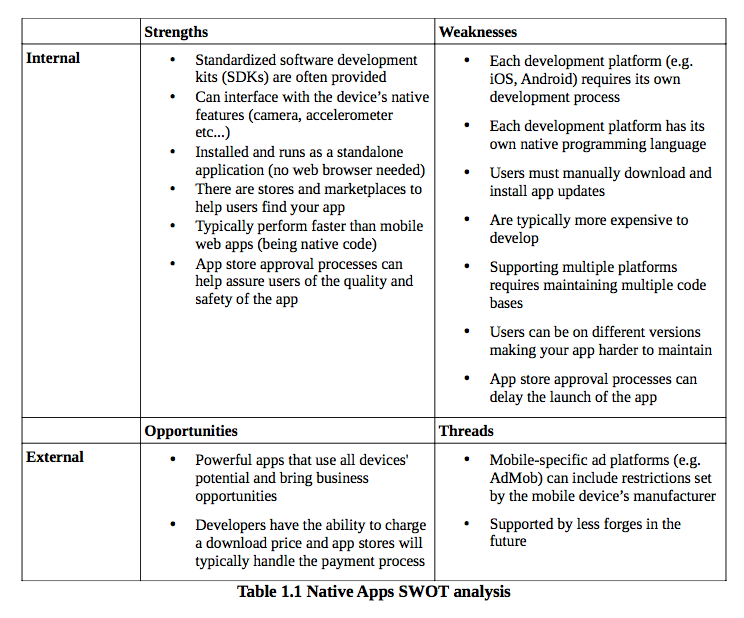
\includegraphics[width=12cm, keepaspectratio]{img/table11.png}
 \end{figure}

The table below summarizes using a SWOT analysis the advantages and disadvantages of Web-based Apps:

\begin{figure}[H]
    \centering
    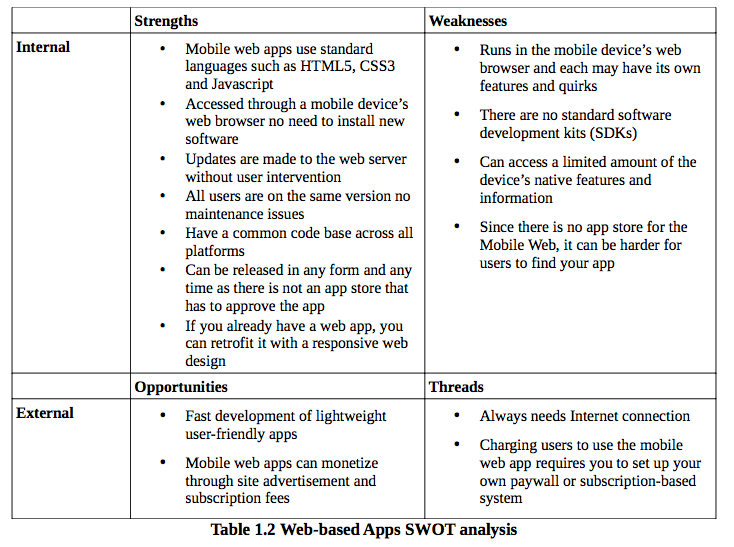
\includegraphics[width=12cm, keepaspectratio]{img/table12.png}
 \end{figure}

To help me decide which type of solution I should take for my KuDo project I asked myself the following questions:

\begin{itemize}
 \item \textbf{Does the mobile app require the use of any special device features (i.e., camera, the camera’s flash, accelerometer, etc.)?} In priciple my idea is to implement simple apps with a high level of responsiveness\footnote{https://en.wikipedia.org/wiki/Responsiveness}  from the user's point of view but the access to the device hardware components is not a must.
 \item \textbf{What is my budget?} Very limited :)
 \item \textbf{Does the mobile app need to be Internet-enabled?} This is not a must for the first applications that I plan to develop in the context of KuDo project but for sure in future versions it would be interesting to be able to link the apps with external educational resources such as Wikipedia, museums, libraries etc...
 \item \textbf{Do I need to target all mobile devices or just certain devices?} Portability is a key issue, the apps should be supported by most of the devices and the idea of having several codebases does not fit within KuDo project.
 \item \textbf{What programming languages do I already know?} Here I have to say that my programming background expertise is more oriented to backend developments and therefore I am ready to start implementing low-level tools using native apps. But on the other side for me it is a good chance to improve my knowledge on web-developments which is a field I cannot explore in my daily professional work.
 \item \textbf{How important is speed and performance?} It is important both using native and web-based apps.
 \item \textbf{How will this app be monetized effectively?} I have some experience in setting up Paypal\footnote{https://www.paypal.com/es/webapps/mpp/home}  systems but I would need some help with this issue; Again, this is an interesting challenge for me.
\end{itemize}

Summarizing, due to the type of developments I am planing to do I think the Web-based Apps solutions (pure web-based or hybrid web-based) are the ones that best fit these purposes even though I am aware that I shall have to make an effort in learning more on HTML5, CSS3, Javascript and other web technologies but I see this as an interesting challenge that shall improve my professional background.

In this Master Thesis I am doing the exercise of performing a deep search in the existing FLOSS Web-based App frameworks for mobile devices, selecting a couple of the most popular ones and then comparing their capabilities using a well-formed quality system like OpenBRR.

% why trade-off using metrics, why OpenBRR, importance of code quality
% ==> MSWL Quality/Evaluation

% por que he elegido FLOSS
% ==> MSWL Licenses
The fact that all frameworks taken under consideration in this study are Open Source solutions is a consequence of different subjects I studied during the Master Thesis and the idea that this kind of solutions bring more benefits to the development community instead of closed solutions.

The objectives of this Master Thesis were defined and agreed with my tutors and can be summarized in the following list:

\begin{itemize}
\item Select a couple of representative Open Source web-based frameworks for developing Mobile Apps from the existing solutions currently available in the market.
\item Set a checklist of points to be analyzed for each solution in the form of well-defined metrics that can be properly measured.
\item Analyze each solution using the OpenBRR methodology, setting different weights and scores for each category according to this model. Spreadsheets shall be used for automating this process.
\item Summarize pros and contras of each solution.
\item Perform a comparison of the results for each solution taking as a baseline the final version of each spreadsheet and also applying a SWOT comparision analysis on top of OpenBRR.
\end{itemize}

%%%%%%%%%%%%%%%%%%%%%%%%%%%%%%%%%%%%%%

\chapter{A first look at the available frameworks}
\label{chap:overview}

\section{Possible candidates}
\label{sec:candidates}
 
There are many web-based frameworks for developing mobile apps nowadays, the first step I performed in this study was to take a deep look in the Internet at the available solutions and select a subset of them that fulfills the requirements of the KuDo project. 
 
\subsection{Appspresso}
\label{Appspresso} 
 
Appspresso\footnote{http://appspresso.com/}  is a hybrid cross-platform mobile framework which wraps source code developed with web technology by each mobile platform runtime and builds them into native mobile apps. Developers can build Apple iOS apps, Google Android apps. Moreover, Appspresso plans in the close future, to support Microsoft Windows Phone, RIM BlackBerry, and Samsung Bada. 

Using only the standard web technologies such as HTML, CSS, and JavaScript, development is easily done  and the existing web-based contents can easily be migrated to apps.

Appspresso is the only mobile framework that supports the device API of WAC (Wholesale Application Community) called Waikiki API\footnote{http://appspresso.com/api-reference}. Waikiki API is a JavaScript API that allows utilization of local resources such as camera, contacts, accelerometer, device status, file system, and etc. The current version Appspresso 1.0 RC supports the Waikiki API 2.0 beta.

Appspresso provides an integrated development environment for Eclipse to develop apps using Appspresso Studio environment regardless of the target mobile platform. With one click of a mouse, iOS and Android apps can be built and WAC apps can be packaged. One of the best things about Appspresso studio, is the possibility to use “on the fly building” function which immediately reflects revised source code without recompiling. Thus improves the development productivity by eliminating the need for rebuilding source code and transferring app to a test mobile or an emulator. 

Appspresso PDK (Plug-in Development Kit) allows developers to use native language to create user-defined functions and expose them through JavaScript API. Waikiki API that is built into Appspresso was also developed using Appspresso PDK. Appspresso runtime provides a plug-in architecture for supporting custom plug-ins and Appspresso Studio includes a PDK necessary for those plug-in developments.

Figure below shows how a simple "Hello World" application would look like:

\begin{figure}[H]
    \centering
    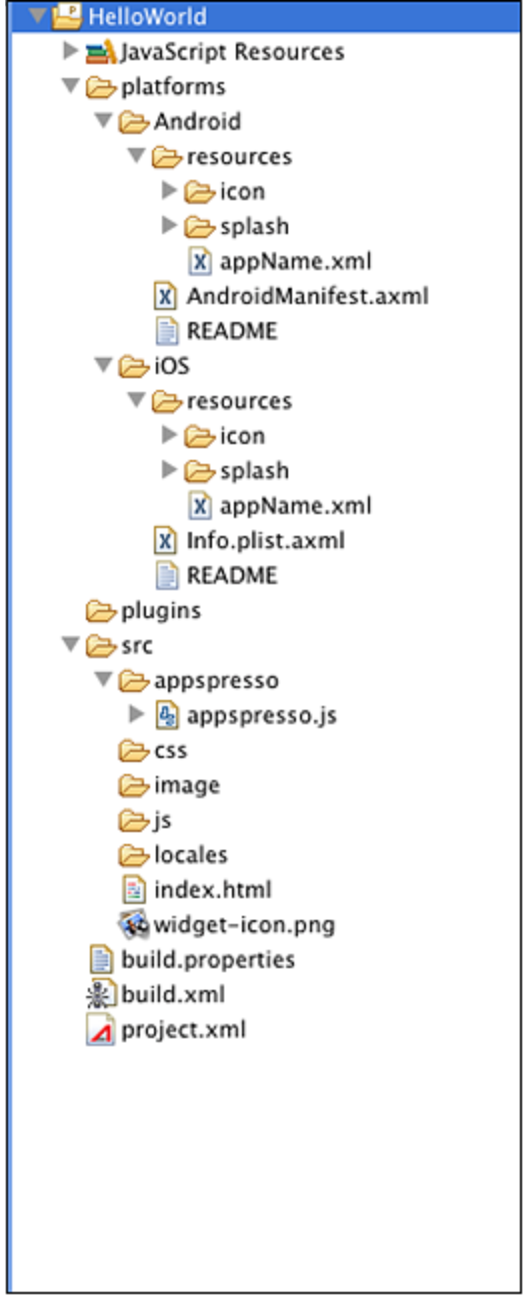
\includegraphics[width=5cm, keepaspectratio]{img/appspresso.png}
    \caption{\textit{Appspresso Hello World example}}
 \end{figure}
 
Appspresso code is maintained using a GitHub repository\footnote{https://github.com/kthcorp/Appspresso-SDK} and it is licensed using a MIT License\footnote{http://opensource.org/licenses/MIT} .
 
\subsection{Sencha Touch}
\label{Sencha Touch}

 % TODO

\subsection{Appcelerator Titanium}
\label{Appcelerator Titanium} 

The Titanium SDK\footnote{http://www.appcelerator.com} lets you develop native, hybrid and mobile web applications from a single codebase. 

Titanium Studio\footnote{http://www.appcelerator.com/platform/titanium-studio/} is an extended version of Aptana Studio, the open source Integrated Development Environment (IDE) tool for web development. In addition to Aptana Studio's web features, Titanium Studio adds the opportunity to develop Appcelerator Titanium Mobile projects, for Android, iOS and Mobile Web. With Titanium Studio it easy to get started to produce professional cross-platform Android, iOS and HTML5-based Mobile Web applications. It includes integrated templates, sample applications and vast amounts of educational material. It helps you to manage the whole project lifecycle of your Titanium projects, including writing, add-on module usage, debugging, integrating with cloud services, through to testing, packaging, and deployment.

\begin{figure}[H]
    \centering
    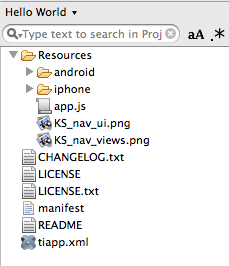
\includegraphics[width=4cm, keepaspectratio]{img/titanium.png}
    \caption{\textit{Titanium Simple Example project structure}}
 \end{figure}

Titanium's unique trait among the various available cross platform mobile solutions is that it creates truly native apps. This is in contrast to web-based solutions that deliver functionality via an enhanced web view. Titanium, not wanting to be limited by the native web view, has engaged in a much deeper integration with the underlying platforms. This gives Titanium developers the ability to leverage native UI components and services, as well as near-native performance, features you won't find in other cross platform mobile development solution. Titanium provides a deep, yet highly-reusable development platform, featuring nearly 100\% code reuse across desktop apps and over 80\% reuse across mobile apps. Appcelerator licenses Titanium under the Apache 2 license\footnote{https://www.apache.org/licenses/LICENSE-2.0.html}  and is free for both personal and commercial use.

At the Titanium web site, we can discover a large number of references and documentation related to some topics such as: UI fundamentals, how to works with local and remote data source, media API use, debugging, distribution, best practices and recommendations, among others. Which is a great guide for beginners and advanced developers.

\subsection{IPFaces}
\label{IPFaces} 

IPFaces\footnote{http://www.ipfaces.org/} is a framework for simple creation of native, form-oriented network applications for mobile devices. The aim of the solution is to screen the programmer completely out from the mobile platform itself, and transfer the entire application logic to central application server level.

Each iPFaces application consists of two main parts: Thin iPFaces client for mobile devices and the server part with application logic and definition of iPFaces views, that basically  is a standard web module. iPFaces provides libraries for easy definition of iPFaces forms for the presentation layer of the application for all supported server platforms (ASP.Net, Java and PHP). The architecture and design logic are not limited in any manner and you may use your usual and tested procedures. 

Figure shows how is the interaction between both sides, generating simple GET/POST requests from the server side by returning iPFaces forms definition in XML format.

\begin{figure}[H]
    \centering
    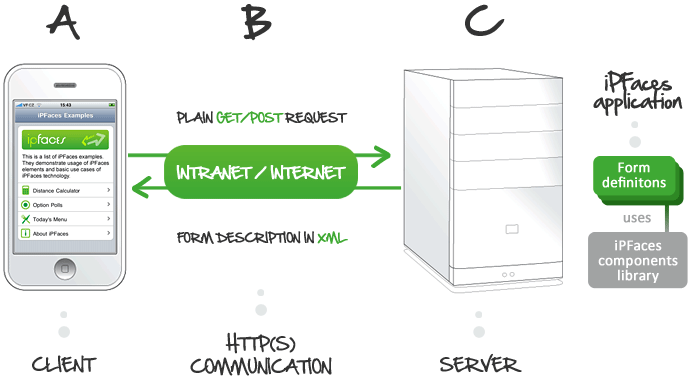
\includegraphics[width=8cm, keepaspectratio]{img/ipfaces.png}
    \caption{\textit{iPFaces Client/Server interaction}}
 \end{figure}

To programming an application for  cross mobile devices with IPFaces, knowledge of specific mobile device platform is not required.  All that we need,  is to install the general iPFaces client to the mobile device in the standard way and file the address of your iPFaces server upon its first launch. The iPFaces client is supplied for free for various mobile platforms as a standard part of the entire solution.

The server part of the iPFaces technology is fully opened, both for non-commercial and commercial use under a BSD licence\footnote{http://opensource.org/licenses/BSD-3-Clause}, more information can be found in the developers site\footnote{http://sourceforge.net/projects/ipfaces/files/1.3/} .

\subsection{MoSync}
\label{MoSync} 

The MoSync\footnote{http://www.mosync.com/}  is an open-source SDK rich environment that make easy to develop cross-platform mobile application for all major mobile platforms from a single code base. The SDK enables mobile developers to build and compile apps for up to nine different platforms at once, using C/C++ or HTML5/JavaScript, or a combination of both to create hybrid apps.

With the MoSync SDK\footnote{http://www.mosync.com/docs/sdk/index.html}  it is possible to build applications with HTML5, JavaScript, and CSS without needing to write a single line of C/C++ code. Also, we can build hybrid apps that use HTML5/JavaScript for the user interface and C/C++ for the heavy lifting. 

The MoSync IDE is based on Eclipse, although there have made several modification in order to make it a great tool for cross-platform mobile application development,  and added  some unique MoSync features. The IDE lets you edit both HTML5/JavaScript (great for defining user interfaces) and C/C++ (ideal for any heavy lifting your app needs to do).

\begin{figure}[H]
    \centering
    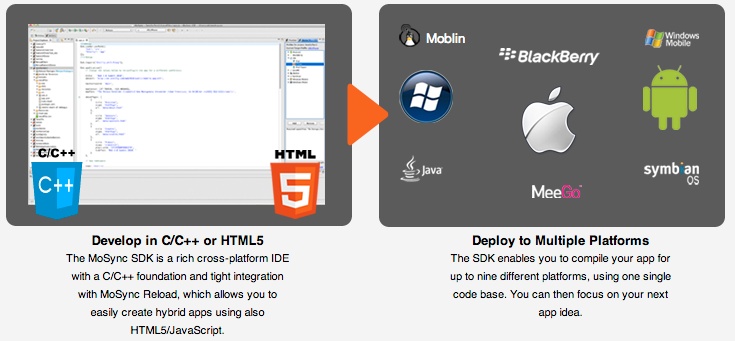
\includegraphics[width=10cm, keepaspectratio]{img/mosync.png}
    \caption{\textit{MoSync IDE based on Eclipse}}
 \end{figure}
 
Also, the MoSync IDE provides a default emulator called  “MoRE”. MoRE is a  virtual machine that directly executes MoSync bytecode and  it allow us to emulate most devices in MoSync's device/platform, including  multitouch emulation. Of course, we can also use native emulators from the IDE, like the Android Emulator and iPhone/iOS Simulator, and run the application in those too.

MoSync JDK is licensed under a GPL v2.0\footnote{https://www.gnu.org/licenses/gpl-2.0.html}  license, the code is available in the corresponding GitHGub repository\footnote{https://github.com/MoSync/MoSync}  and more information can be found in the project developers web site\footnote{http://www.mosync.com/docs/index.html} .

\subsection{jQuery Mobile}
\label{jQuery Mobile}

\subsection{Cordova}
\label{Cordova} 

Apache Cordova\footnote{https://cordova.apache.org/} is a set of device APIs that allow a mobile app developer to access native device function such as the camera or accelerometer from JavaScript. Also, combined with a UI framework such as jQuery Mobile or Dojo Mobile or Sencha Touch, this allows a smartphone app to be developed with just HTML, CSS, and JavaScript.

When using the Cordova APIs, an app can be built without any native code (Java, Objective-C, etc) from the app developer. Instead, web technologies are used, and they are hosted in the app itself locally (generally not on a remote http server). And because these JavaScript APIs are consistent across multiple device platforms and built on web standards, the app should be portable to other device platforms with minimal to no changes.
Apps using Cordova are still packaged as apps using the platform SDKs, and can be made available for installation from each device's app store.

Cordova provides a set of uniform JavaScript libraries that can be invoked, with device-specific native backing code for those JavaScript libraries. Cordova is available for the following platforms: iOS, Android, Blackberry, Windows Phone, Palm WebOS, Bada, and Symbian.

Apache Cordova graduated in October 2012 as a top level project within the Apache Software Foundation (ASF). Through the ASF, future Cordova development will ensure open stewardship of the project. The project is licensed using the Apache Public License (APL) 2.0\footnote{https://www.apache.org/licenses/LICENSE-2.0.html} , more information can be found in the project contributors web site\footnote{https://cordova.apache.org/\#contribute} .

\subsection{Dojo Mobile}
\label{Dojo Mobile} 

Dojo Mobile\footnote{http://dojotoolkit.org/features/mobile}  is a HTML5 mobile JavaScript framework that enables rapid development of mobile web applications with a native look and feel on modern webkit-enabled mobile devices such as iPhone, iPod Touch, iPad, Android and RIM smartphones and tablets.

The framework provides the following capabilities:
\begin{itemize}
\item Includes a new set of components designed from scratch with mobile in mind, including forms and databinding. Switches, Sliders, Lists, Actions etc.
\item Is integrated with the new MVC and Application Controller packages.
\item Mobile themes are optimized for performance, using the latest techniques, such as CSS3 icons. Themes are built using CSS and parameterized using Less.js, making it very easy to change styling such as colors across an entire theme in one place — including graphical components such as charts and gauges.
\item Comes with default themes for iOS, Android and Blackberry out of the box for the core mobile widgets, so you can match the native look and feel that users are already accustomed to working with.
\item There are specific Dojo plugins for the most common IDEs in the market, the most popular is the one integrated in Aptana/Eclipse\footnote{http://dojotoolkit.org/features/tools} . 
\item When you want to utilize app stores for marketing, your Dojo Mobile app can easily be packaged as a native app using PhoneGap, a quality open source affiliate project with similar licensing.
\end{itemize}

Figure below shows an example of development using Dojo Mobile toolkit:

\begin{figure}[H]
    \centering
    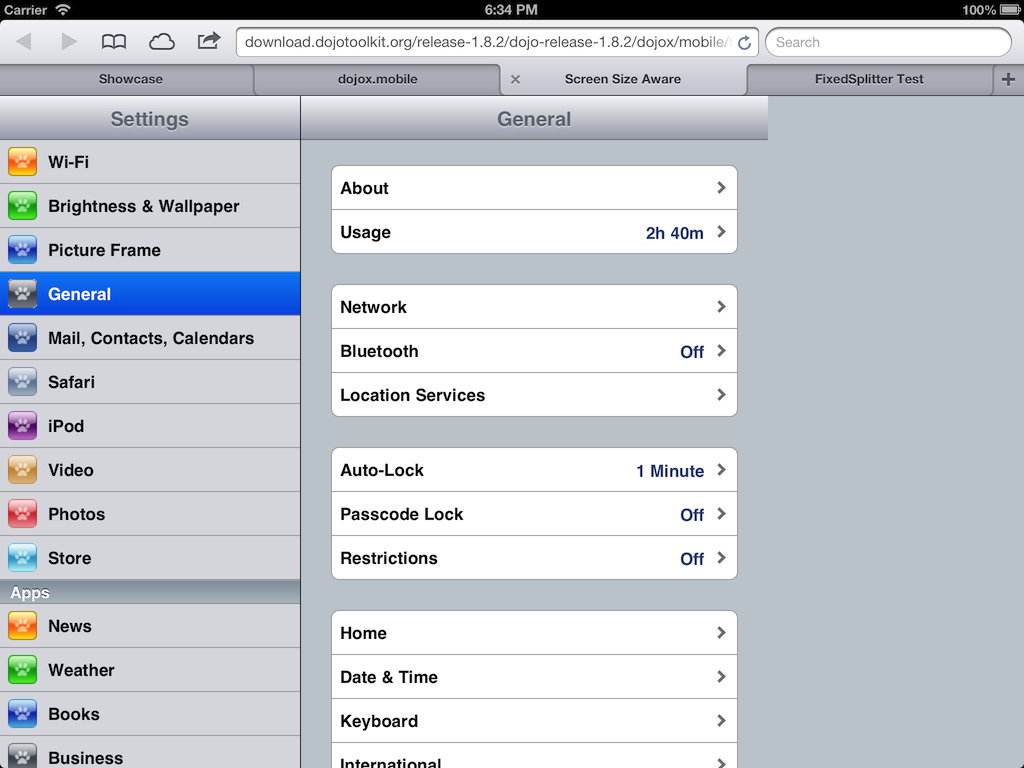
\includegraphics[width=10cm, keepaspectratio]{img/dojo.png}
    \caption{\textit{Dojo Mobile toolkit example}}
 \end{figure}

The project is hosted by the Dojo Foundation\footnote{http://dojofoundation.org/mobile}, and the mobile toolkit is licensed under BSD and Academic Free License (AFL) v3.0\footnote{http://opensource.org/licenses/AFL-3.0} open source licenses. More information can be found in the project Community web site\footnote{http://dojotoolkit.org/community/} .

\section{Selected frameworks}
\label{sec:selected}
Taking this list as a baseline then




%%%%%%%%%%%%%%%%%%%%%%%%%%%%%%%%%%%%%%


\chapter{OpenBRR Analysis}
\label{chap:openbrr}

\section{What is OpenBRR?}
\label{sec:openbrr2}

The Business Readiness Rating model (OpenBRR)\cite{OpenBRRWhitepaper} is
intended to help IT managers assess which Open Source software would be most suitable for their needs. Open Source users can also share their evaluation ratings with potential adopters, continuing the virtuous cycle and “architecture of participation” of open
source.

The initiative\cite{The OpenBRR Corporate Community}  is lead by the Carnegie Mellon West University, Spike Source, Intel and O’Reilly’s Code Zoo and offer proposals for standardizing different types of evaluation data and grouping them into categories.

The framework suggests the following metrics to be analyzed and evaluated:
\begin{itemize}
\item Functionality
\item Usability
\item Quality
\item Security
\item Performance
\item Scalability
\item Architecture
\item Support
\item Documentation
\item Adoption
\item Community
\item Professionalism
\end{itemize}

The model is composed of the following phases:
\begin{itemize}
\item Phase 1 - Quick Assessment: defining and ranking of metrics and categories according to their importance within the product that is going to be evaluated.
\item Phase 2 - Target usage assessment: Set the necessary category and metric weights according to the project's goals.
\item Phase 3 - Data collection and processing: Gather data for each metric used in each category rating, and calculate the applied weighting for each metric, spreadsheets are used for this purpose.
\item Phase 4 - Data translation: Use category ratings and the functional orientation weighting factors to calculate the Business Readiness Rating score and publish the software’s Business Readiness Rating score.
\end{itemize}

The Business Readiness Rating model offers a trusted and open framework for software evaluation, this model aims to accelerate the software evaluation process with a systematic approach, facilitate the exchange of information between IT managers, result in better decisions, and increase confidence in high-quality open source software.

\section{Data Sources}
\label{sec:data}

For analyzing the different web-based mobile app frameworks and provide a reliable comparison, data from different primary/secondary sources will be used. In this section I present the most important ones; other sources will be referenced or explained directly (for example using a footnote) when the corresponding fact, metric or argument is discussed.

The starting point for getting data on the selected solutions are the official websites of jQuery Mobile\cite{jquery} and Sencha Touch\cite{sencha}, they provide reliable information about their functionality, history, documentation and support. 

One of the data sources we studied in the MSWL was Ohloh\cite{Ohloh} which is a free public
directory of open source software and people, owned and operated by BlackDuck Software Inc., a consulting company specialized in gathering and providing information about open source software projects. Metrics present in Ohloh site are provided by Ohloh specific tools and others are provided by gathering the information provided by Ohloh users for their own projects or the projects they are interested in.

Both jQuery Mobile and Sencha Touch are sub-projects of other parent projects (jQuery and Sencha), in Ohloh we can find information about both the parent and child projects:

\begin{itemize}
 \item For jQuery Mobile there is a dedicated page in Ohloh\cite{ojquery} that provides very valuable information about the project for our trade-off analysis. Also the parent project jQuery\cite{ojqueryparent} and other related extensions have their own pages in Ohloh data source.
 \item For Sencha Touch the situation is not the same. Even though we can find an entry in Ohloh for the parent Sencha project\cite{osencha}, the page has no activity since a long time. Therefore unfortunately we cannot take Ohloh as data source for finding information in the case of Sencha Touch, because its code reposiroty is not open to the public and we shall have to use other sources.
\end{itemize}

In the MSWL we studied other data sources like FLOSSMetrics\cite{FLOSSMetrics}, FLOSSmole\cite{FLOSSmole} and FLOSShub\cite{FLOSShub} which provide centralized access to data analysis (charts, tables and other quantitative information) of free/libre/open source projects hosted in forges such as Sourceforge\footnote{https://sourceforge.net/}, GForge\footnote{http://gforge.org/gf/} etc... Also we saw that the FLOSSpapers project\cite{FLOSSpapers} allows to perform queries on papers published on these purposes.

Unfortunately because the technologies we are studying in this thesis are quite new, there is no data for both jQuery Mobile and Sencha Touch project in none of the data sources cited above, so I had to look for other sources of information.

One of the most interesting data sources nowadays is LinkedIn\footnote{https://www.linkedin.com/},  a social networking website for exchanging profesisonal information, where there are lots of groups devoted to mobile apps technologies. I have performed a seach in several of those groups looking for information on jQuery Mobile and Sencha, specially in the "iPhone, Android, iPad, Tablet \& Mobile Application Development"\cite{linkedin1},  the "Mobile Software Development Group"\cite{linkedin2} and the "Developers HTML5, Android, iOS, Windows, Java, BlackBerry"\cite{linkedin3} groups which are very active. LinkedIn allows users to start discussions and polls in the groups they are subscribed to. 

Another interesting tool I have discovered during my thesis is Survey Monkey\footnote{http://es.surveymonkey.com/}, a tool for publising quite complete polls for free, the system is more complete than other solutions like the LinkedIn polls system.

Also for searching information on some metrics included in this trade-off study, I have used Quora\footnote{https://www.quora.com/}  wuich is a question-and-answer website which lots of information on the mobile web apps field.

Also Google discussion groups\footnote{https://groups.google.com} which contain a searchable archive of more than 700 million Usenet postings from a period of more than 20 years is a valuable source of information.

A good resource for searching useful articles about mobile web apps development (and in general any kind of development technologies) is the IBM Developer Works site that has dedicated sections for different frameworks like Dojo JS\footnote{https://www.ibm.com/developerworks/topics/dojo}, jQuery Mobile\footnote{http://www.ibm.com/developerworks/topics/jquerymobile}, PhoneGap\footnote{https://www.ibm.com/developerworks/topics/phonegap}, Sencha Touch\footnote{http://www.ibm.com/developerworks/topics/sencha\%20touch}  etc...	 

Regarding books available for each project, Amazon\footnote{http://www.amazon.com} is the reference data source I have used.

Regarding demos/presentations, I have used Slideshare as main data source. There are many resources available for jQueryMobile\footnote{http://www.slideshare.net/search/slideshow?searchfrom=header\&q=jquery+mobile}  and Sencha Touch\footnote{http://www.slideshare.net/search/slideshow?searchfrom=header\&q=sencha+touch}  there.

Also for having a better idea on measuring some of the metrics related to the functionalities provided by each framework, like how easy is the installation process, available IDEs, portability to different mobile devices etc... I have developed a couple of prototype examples: one for jQuery Mobile and another for Sencha Touch. The source code of these examples can be found in the thesis Github repository under:\\

\url{https://github.com/eparrillae/eparrillae-mswl-thesis/tree/master/MasterThesis/prototypes}

%%%%%%%%%%%%%%%%%%%%%%%%%%%%%%%%%%%%%%

\chapter{Trade-Off Results}
\label{chap:results}

As stated before, I am going to follow the "Business Readiness Rating for Open Source
(OpenBRR)" whitepaper\cite{OpenBRRWhitepaper} to apply this model to the evaluation of the different solutions I have selected: jQuery Mobile and Sencha Touch.

\section{Phase 1: Quick Assessment}
\label{sec:phase1}
This first phase is focused in setting the number of categories used and the different metrics that shall be evaluated per category. The canonical OpenBRR model recommends to focus in not more than seven categories, but in order to provide a more general overview, I have considered the twelve categories present in the model.

Regarding the metrics, I have reviewed the list of metrics provided by the canonical OpenBRR model template. If these metrics fit well with the type of tools I have to analyze (mobile web app) I have left them as they are but in some cases I have substituted the default metrics with new ones that measure better the quality of the products.

\subsection{Functionality Category metrics definition}
\label{Functionality Category metrics definition}

The most important category within this study is the "Functionality" category, here I have defined a set of very specific criteria to evaluate precisely the selected frameworks. To be able to define a complete subset of metrics I have used two different sources:

\begin{itemize}
 \item The experience analyzing the available solutions in the market for developing mobile web apps done in previous section "Selected Frameworks".
  \item The experience developing jQuery Mobile and Sencha Touch prototypes.
 \item Wikipedia comparison tables between web-based mobile app frameworks \cite{wikipedia1}  and HTML5/CSS3/Javascript frameworks \cite{wikipedia2}.
\end{itemize}

\subsection{OpenBRR improvements with new metrics}
\label{OpenBRR improvements with new metrics}

The following new metrics have been added to this study:

\subsubsection{Multiplatform support}
\label{Multiplatform support}

I have added this metric in the \textbf{Usability} category. One of the key points of the development of KuDo projects is that the applications can be run in the most popular mobile platforms used nowadays. Therefore, it is quite important to ensure that the selected framework runs well in different web browsers and mobile devices containing those web browsers.

The score assigned to this metric will be:
\begin{itemize}
 \item Good Support: 5
 \item Regular Support: 3
 \item Poor Support: 1
\end{itemize}

\subsubsection{Is there a dedicated information (web page, wiki, etc) for security?}
\label{Is there a dedicated information (web page, wiki, etc) for security?}

I have added this metric in the \textbf{Security} category, even though security is not a key aspect for the KuDo project, because the applications that shall be deployed are going to be very simple ones with no authentication procedures it is always interesting which support is provided by default.

The score assigned to this metric will be:
\begin{itemize}
 \item Yes, well maintained: 5
 \item Yes: 3
 \item No: 1
\end{itemize}

\subsubsection{Architecture based on design patterns}
\label{Architecture based on design patterns}

I have added this metric in the \textbf{Scalability} category. The idea is to check if the selected framework is built on top of a robust architecture that can be extended in the future. For that reaosn the usage of design patterns is so important.

The score assigned to this metric will be:
\begin{itemize}
 \item Yes, architecture fully based on standard design patterns: 5
 \item Yes, partially: 3
 \item No: 1
\end{itemize}

\subsubsection{Are there any repositories of 3rd party UI Plug-ins}
\label{Are there any repositories of 3rd party UI Plug-ins}

I have added this metric in the \textbf{Architecture} category. For any kind of user interface development it is quite important to have a good toolkit of UI widgets coming by default with the selected solution, but also if there are external repositories containing widgets implemented by 3rd party developers, this helps a lot in extending the capabilities provided by the applications.

The score assigned to this metric will be:
\begin{itemize}
 \item More than 5 repositories available: 5
 \item 1 to 5 repositories available: 3
 \item 1 repositories available: 1
\end{itemize}

\subsubsection{Backend Services Support}
\label{Backend Services Support}

I have added this metric in the \textbf{Architecture} category. The idea is to measure the availability of pluggable backend libraries for connecting with databases, external file systems, web services etc...

The score assigned to this metric will be:
\begin{itemize}
 \item Yes, extensive: 5
 \item Yes: 3
 \item No: 1
\end{itemize}

\subsubsection{Enable/disable features through configuration}
\label{Enable/disable features through configuration}

I have added this metric in the \textbf{Architecture} category. The idea is to measure how easily the framwork can be configured.

The score assigned to this metric will be:
\begin{itemize}
 \item Yes, during runtime: 5
 \item Yes, during runtime: 3
 \item No: 1
\end{itemize}

\subsubsection{Programming Languages}
\label{Programming Languages}

I have added this metric in the \textbf{Architecture} category. As we saw during the "Communities" subject of the MSWL, for a given development the support of more languages in the core source code of the framework means more flexiblity and also more people may get involved in the project. If the project is completely built based in just one programming language it is possible that a developer who does not know about the language used on it cannot collaborate.

But also is important the amount of code used in a concrete programming language, it would not be good if we say that a FLOSS project uses three different programming languages when one of them just has a few lines of code.

The score assigned to this metric will be:
\begin{itemize}
 \item 80\% or more of SLOC in three or more languages: 5
 \item 80\% or more of SLOC in two languages: 3
 \item 80\% or more of SLOC in one language: 1
\end{itemize}

\subsubsection{Framework web site quality}
\label{Framework web site quality}

I have added this metric in the \textbf{Documentation} category. A good web site should provide a centralized point for getting information on the project's objectives, license, access to source code, forums, mailing lists, etc..

Also the information should be provided for the various end-users roles: 
\begin{itemize}
 \item users with no experience using mobile app frameworks
 \item users with experience using mobile app frameworks but with no experience using this particular framework
 \item developers of the framework
 \item project administrators
\end{itemize}

The score assigned to this metric will be:
\begin{itemize}
 \item Superb web site: 5
 \item Acceptable web site: 3
 \item Poor web site: 1
\end{itemize}

\subsubsection{Longevity}
\label{Longevity}
A new metric is introduced in the \textbf{Community} category. I think that the longevity of a given project must be measured combining two different criteria. In one hand the project's age, but also it has to be analyzed if during the whole project lifecycle there has been development activity, a very old project with just a few activity is really useless for the KuDo project purposes.

Taking into account the previous assertions, the normalized scores to assign to this metric will be:
\begin{itemize}
 \item Young project (more than 1 year old) and increasing lines of code production : 1
  \item Medium project (more than 5 years old) and increasing lines of code production : 3
 \item Long project (more than 10 years old) and increasing lines of code production: 5
\end{itemize}

\subsubsection{Cloud Support}
\label{Cloud Support}
A new metric is introduced in the \textbf{Community} category. This metric is related with the feature to provide backend-as-a-service capabilities that allows developers to access a set of APIs that helps them to build, run and test their applications in a cloud environment.

The score assigned to this metric will be:
\begin{itemize}
 \item Full support: 5
  \item Partial Support : 3
 \item No Support: 1
\end{itemize}

\subsubsection{License}
\label{License}

A new metric is introduced in the \textbf{Professionalism} category. For the KuDo project it is a must that the mobile app solutions is licensed under an OSI-approved\footnote{http://www.opensource.org/licenses} FLOSS license. Also if the license allows to mix the product with proprietary code is an enhancement.

Taking into account the previous assertions the normalized scores to assign to this metric will be:
\begin{itemize}
 \item Non-OSI-Approved license: 1
 \item OSI-Approved and "copyleft"\footnote{https://www.gnu.org/copyleft/} license: 3
 \item OSI-Approved and "weak copyleft/permissive"\footnote{https://en.wikipedia.org/wiki/Permissive\_free\_software\_licence}  license: 5
\end{itemize}

\section{Phase 2: Target Usage Assessment}
\label{sec:phase2}
This second phase consists in setting the category and metric weights according to the KuDo project requirements. The canonical OpenBRR model recommends to focus in not more than seven categories, but as I said before, in order to provide a more general overview, I will consider the twelve categories present in the model.

If we were considering all the categories equal in importance, we should weight each one of them with 8,33\%. Our assessment will consider this number, in order to weight more than 8\% the categories considered relevant for the KuDo project needs, and less than 8\% the categories considered not so relevant.

The most important selected categories have been \textbf{Functionality} and \textbf{Usability}. Each one of them have been given a weight of 12\%, so together they reach 24\% of the total evaluation.

The OpenBRR model provides no ready-to-collect metrics for \textbf{Functionality}, allowing the evaluator to create them in a tailored way according to the customer's requirements. In the previous section "Functionality Category metrics definition", I have explained the criteria followed to define the list of metrics.

\textbf{Support}, \textbf{Documentation} and \textbf{Community} are also desirable aspects, that ensure the liveness of the community of any piece of software, and also guarantee usability since good instructions and advices smooth out the
difficulties of any tool. For this reason these categories have been
weighted with 10\%. 

With the same arguments, I have evaluated \textbf{Adoption}, but we also need to know that there are two influent factors in adoption: on one hand, we need time for any tool to be widely used. On the other hand, "trends" have also influence in the IT world; and certain
companies or tools come in a particular time to the crest of the wave, but quickly sink into obscurity due to the dynamism of the technologies environments. 

\textbf{Architecture}  and \textbf{Scalability} are also key aspects of this trade-off, as I am looking for a framework that serves as a baseline for the developments done in the context of the KuDo project, this framework should provide an architectural design modular and flexible enough to allow the integration of new components to the "core" in an easy way.

About \textbf{Quality}, \textbf{Security} and \textbf{Performance} the given weight has been 5\%, as I have not defined yet strong requirements on this purpose, but they desirable features specially for the future of the project when the mobile apps to be developed become more and more complex.

Finally \textbf{Professionalism} has been given a weight of 5\%. It is important that the selected framework is supported by a robust community and in the particular case of jQuery Mobile and Sencha Touch both are sub-projects that were created from a bigger parent project (jQuery and Sencha) which ensures its stability. 

In conclusion, in table below I present the categories and
their resulting weights for our evaluation.

\begin{table}[ht]
\begin{center}
    \captionof{table}{OpenBRR Target Usage Assessment for web-based Mobile App Frameworks}
    \begin{tabular}{ | l | c | r |}
    \hline
    \textbf{Rank} & \textbf{Category} & \textbf{Weight} \\ \hline
    1 & Functionality & 12\% \\ \hline
    2 & Usability & 12\% \\ \hline
    3 & Quality & 5\% \\ \hline
    4 & Security & 5\% \\ \hline
    5 & Performance & 5\% \\ \hline
    6 & Scalability & 8\% \\ \hline
    7 & Architecture & 8\% \\ \hline
    8 & Support & 10\% \\ \hline
    9 & Documentation & 10\% \\ \hline
    10 & Adoption & 10\% \\ \hline
    11 & Community & 10\% \\ \hline
    12 & Professionalism & 5\% \\ \hline
     & \textbf{TOTAL WEIGHT} & \textbf{100\%} \\ \hline  
    \end{tabular}
\end{center}
\label{OpenBRR2}
\end{table}

\section{Phase 3: Data collection and processing}
\label{sec:phase3}
For filling the differents scores assigned to each category defined previously I have used the OpenBRR baseline spreadsheet provided to the students of Master on Libre Software 2011-2012 located at:\\
\url{http://docencia.etsit.urjc.es/moodle/mod/resource/view.php?id=4350}

For more information about this topic you can visit the MSWL Project Evaluation Subject's Moodle site in:\\
\url{http://docencia.etsit.urjc.es/moodle/course/view.php?id=125}. 

This spreadsheet has an initial set of metrics for each OpenBRR category, allowing to ponderate each metric and providing a normalized score according to the possible values obtained in measurements.

Category weights have been introduced in the sheets. Each metric within each category should have a weighting factor to differentiate the metric's importance withing that particular category. 

Each metric has been measured searching the Internet and getting the needed information from official mailing lists or websites and referencing that link in the corresponding "Raw score" cell with a "comment" in the cell. When a reference is not provided, it means that that metric could not be found or the own tool command line help or main website announces that aspect so it is easy to find.

For the unknown data, I have assigned the worst possible normalized score to the corresponding metric, so the results is not biased by unreliable information.

\section{Phase 4: Data Translation}
\label{sec:phase4}

After collecting all the data and normalizing using the OpenBRR spreadsheet, scores for each category and a global score is automatically calculated.

The resulting work is summarized in the following subsections:

\subsection{jQuery Mobile Results}
\label{jQuery Mobile Results}

The OpenBRR spreadsheet containing the metrics final scores and comments justifying those scores can be found here:

\url{
https://github.com/eparrillae/eparrillae-mswl-thesis/blob/master/MasterThesis/thesis/OpenBRR_Templates/BRR_Template_jQueryMobile.ods}

The final score for jQuery Mobile is 4.0015, which is a very high score. That means that this framework covers most of the needs required for the KuDo development project.

In the \textbf{Functionality} category we can see that most of the requirements are covered, the framework seems to be strong in areas like easy to install and use, multiplatform support, compliance with HTML, CSS3 standards for the web, themes customization and availability of 3rd party plugins/extensions. Also the development environment which is a key part of the implementation process is fully covered, even though there is no dedicated plugin for Eclipse IDE which is the one I use it is possible to do this integration through Aptana IDE\footnote{http://stackoverflow.com/questions/4721124/how-to-enable-jquery-support-in-aptana-studio-3} .

The weakest points in the case of functionality metrics are located in the access to native features of the mobile device that has to be done through other tools like\footnote{http://phonegap.com/} and the support of some advanced features like media audio/video and look\&feel stencils which is very poor at the moment.

In the \textbf{Usability} category, again, we can see that the framework is easy to install and use in a wide range of devices. This is very important for the KuDo project, portability problems could be an issue and the selected solution should cope with that in the proper way.

For measuring the \textbf{Quality} category metrics we have accessed jQuery Mobile GitHub repository\cite{jQuery Mobile Github repo} where we can find useful information about developers involved in the project, project milestones and roadmap, bugs/enhancements raised in the code, etc..

In terms of major releases jQuery Mobile is in the range of 1 to 3 major releases which means that the project is active, but its community is not very big yet. The latest release is from the 20th of February 2013 (v1.3.0) so we have a very recent version to be downloaded and installed.

The activity of fixing bugfixes in the code repository that is measured by the rest of metrics in this category clearly show that the jQuery Mobile community is alive. This is very important for the KuDo project as I would like to take a baseline solution which is alive and garantees the close future of the project.

In the \textbf{Security} category, we can see in Github repo\footnote{https://github.com/jquery/jquery-mobile/issues?labels=4+-+High\&page=1\&state=open}  that there are no major open issues in terms of security. The framework is very simple and there are no specific packages dedicated to security. Also in this category we have the new metric that checks if there is a dedicated web page for security issues, we see that there are no specific documentations on this regard.

In the \textbf{Performance} category we see some of the weakest points of this framework. There are no formal reports about the performance of the framework in different devices, also jQuery does not provide any benchmark/sandbox for testing purposes, which means that the developer itself shall have to write the proper unitary/integration tests from scratch which is a clear pitfall of this solution. Also I could not find any wide documentation about tunning performance, for that reason this framework has slow scores in this category.

In the \textbf{Scalability} category, it is clear that jQuery Mobile is based on a pluggable architecture which is quite extensible but the usage of standard design patterns is not provided by default just the Abstract Factory design pattern is used for its UI widgets toolkit. Other patterns should be built by yourself from scratch like for example the implementation that the M Project\footnote{http://www.the-m-project.org/}  has done.

In the \textbf{Architecture} category, we see that there is a wide range of 3rd party plugins and extensions\cite{jQuery Mobile resources} available which is quite importante for the KuDo project. Unfortunately most of those resources are related with the presentation layer of the applications and the support for plugins to connect backend services such as databases, web services, etc.. is not fully covered. 

In terms of programming languages, figure below shows the results of executing SLOC\footnote{http://www.dwheeler.com/sloccount/} over jQuery Mobile code in the Ohloh statistics page:

\begin{figure}[H]
    \centering
    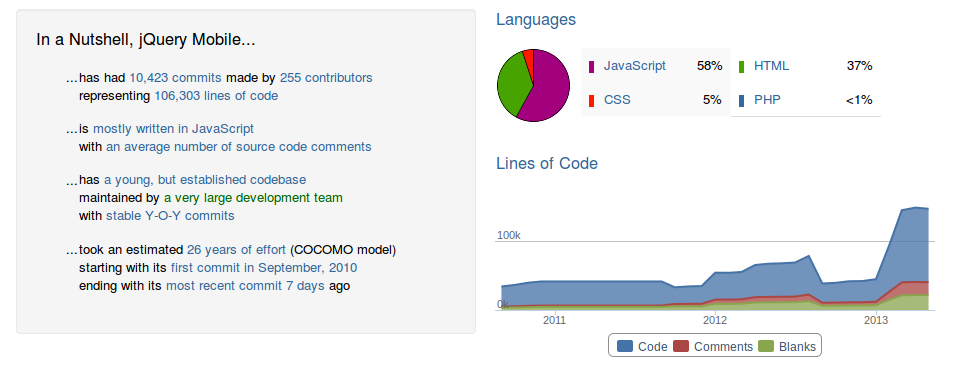
\includegraphics[width=15cm, keepaspectratio]{img/jquerylanguages.png}
    \caption{\textit{jQuery Mobile Programming Languages}}
    \label{figure:jquerylanguages}
 \end{figure}

We see that most of the code is done using Javascript/HTML, which means that for implementing mobile apps using this framework requires a huge background experience in these languages, this could be a challenge for me as my experience is not so deep in that field.

In the \textbf{Support} category we can clearly see that the jQuery Mobile community is very active and the mailing lists work very well. But if we are looking for any kind of professional support that capability is missing within the project, for that reason we conclude that for using jQuery Mobile as baseline for KuDo developments it is necessary to have some background in web-based software development.

Regarding the \textbf{Documentation} category, I have to say that the project is really well-documented, there are lots of books about jQuery Mobile and the web site contains all necessary resources for both developers without experience and advanced ones, in this category all scores are high. This applies also for the \textbf{Adoption} category, there are many real-world examples of mobile apps developed using jQuery Mobile framework.

In the \textbf{Community} category, we see that average volume of messages in the mailing lists in the last six months is high, also the number of commits in the last month is good but the number of contributors in this period is still low as shown in figure below:

\begin{figure}[H]
    \centering
    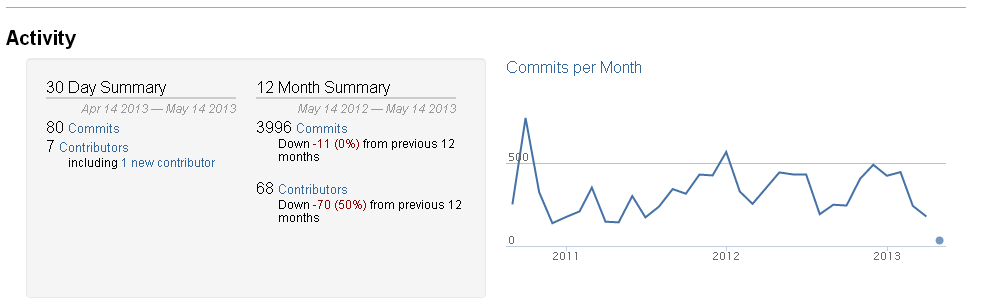
\includegraphics[width=15cm, keepaspectratio]{img/jqueryohloh.png}
    \caption{\textit{jQuery Mobile Monthly Statistics in Ohloh}}
    \label{figure:jquerymonthly}
 \end{figure}
 
The fact that the number of contributors to the 'core' is still low can be a problem to guarantee the sustainability of the project in the future and must be taken into account.

In terms of Longevity, jQuery is considered still a young project, but taking into account that it is supported by its parent project jQuery\footnote{http://jquery.com/}  managed by the jQuery Foundation\cite{jQuery Foundation} which is very active and I think the future of the project is ensured.

In the \textbf{Professionalism} category, the role of the jQuery Foundation is crucial for organizing conferences and workshops that promote the framework among its users community (the next jQuery Conference to be held in June 2013\footnote{http://events.jquery.org/2013/portland/}).

Also the community around jQuery Mobile is very welcome to receive new contributors\footnote{http://forum.jquery.com/topic/how-can-i-contribute-to-jquery-mobile-core-development} which makes the process of participating in the project easier which is something I would really like to do.

Finally jQuery Mobile is licensed under a MIT license\footnote{http://opensource.org/licenses/MIT} which is perfect for KuDo project purposes. My idea is to integrate in jQuery Mobile other open source plugins and also implement on top of the framework my own developments.

The table below summarizes using a SWOT analysis, the advantages and disadvantages of jQuery Mobile after the OpenBRR analysis:

\begin{figure}[H]
    \centering
    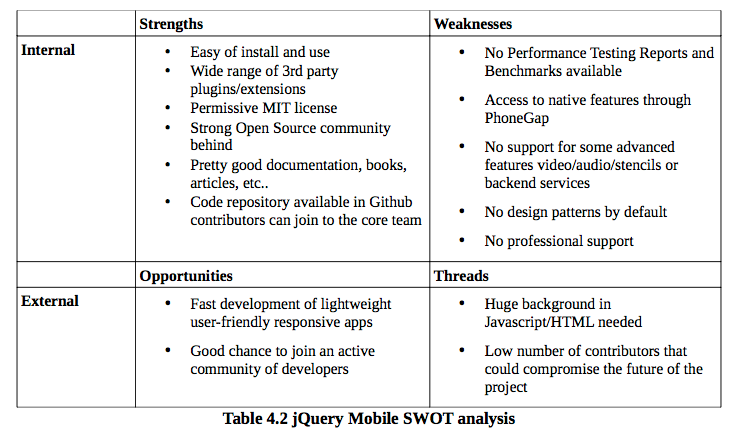
\includegraphics[width=12cm, keepaspectratio]{img/table42.png}
 \end{figure}

\subsection{Sencha Touch Results}
\label{Sencha Touch Results}

The OpenBRR spreadsheet containing the metrics final scores and comments justifying those scores can be found here:

\url{
https://github.com/eparrillae/eparrillae-mswl-thesis/blob/master/MasterThesis/thesis/OpenBRR_Templates/BRR_Template_SenchaTouch.ods}

The final score for Sencha Touch is 3.723, which is a lower score than the one we got for jQuery Mobile. That means that this framework covers many of the needs required for the KuDo development project but it is not as complete as jQuery Mobile.

In the \textbf{Functionality} category, we can see that most of the requirements are covered. The framework seems to be strong in areas like easy to install and use, compliance with HTML, CSS3 standards for the web, themes customization and availability of 3rd party plugins/extensions. 

Also the development environment which is a key part of the implementation process is fully covered. In the case of Sencha, there is a dedicated plugin for Eclipse IDE\cite{sencha Eclipse Plugin}  which makes easier the development as this is the IDE I am used to use. Also Sencha Touch provides Sencha Architect\cite{sencha Architect} which is a tool that provides sketching and drag\&drop graphical desing features.

One important pitfall for Sencha Mobile is that it is focused on running well in Webkit\footnote{https://www.webkit.org/}  based web browsers, for that reason multiplatform support in Black Berry and Nokia devices is not guaranteed.

Also the access to native features of the mobile device that has to be done through other tools like PhoneGap\footnote{http://phonegap.com/} which is the same case we had in jQuery Mobile. 

On the other hand, the support of some advanced features like media audio/video and look\&feel stencils is fully supported in Sencha Mobile.

Sencha Mobile supports by default a MVC architecture\cite{sencha MVC}  that makes easier the development of well-structured mobile apps.

In the \textbf{Usability} category, we get similar scores that the ones for jQuery Mobile, we can see that the framework is easy to install and use.

For measuring the \textbf{Quality} category metrics, we have checked that in Ohloh we do not have specific information about Sencha Touch\cite{Ohloh Sencha Touch}. This is because the code repository of Sencha Touch is not open to the public, this is a big difference with jQuery Mobile where there is a GitHub project where we can check the source code improvements, bugs/enhancements raised and their status etc... This point is one of the reasons that have made Sencha Touch to be evaluated lower that jQuery Mobile in this category. Without the repository it has been impossible to score the required metrics, for that reason those metrics have the lowest score possible.

In terms of major releases Sencha Touch is in line with jQuery Mobile both are in the range of 1 to 3 major releases which means that the project is currently active, the latest release is from the 15th of April 2013 (v2.2.1) so we have a very recent version to be downloadable and installed. Here we have to say that Sencha Touch has delivered more stable releases than jQuery Mobile, therefore it seems that the number of companies/developers behind the project could be bigger than the jQuery Mobile community.

In the \textbf{Security} category, again we cannot check the number of critical bugs open in the Sencha Touch code and its status. Therefore those metrics are scored with the lowest possible value. Like in jQuery Mobile, Sencha Touch does not have a dedicated package for security.

In the \textbf{Performance} category there are differences with jQuery because Sencha does provide tools for benchmarking and testing our mobile apps and also provides formal performance comparisons (see benchmarking results in \cite{sencha performance}). This is a strong point in favour of Sencha, because jQuery Mobile does not provide anything on this regard.

In the \textbf{Scalability} category, Sencha Touch is based on a pluggable architecture which is quite extensible and also the usage of standard design patterns is  provided by default (see usage of MVC \cite{sencha MVC}) which is a difference with jQuery. So here the scores for the different metrics are the highest possible.

In the \textbf{Architecture} category, we see that there is a wide range of 3rd party plugins and extensions (see Sencha Try site \cite{sencha Try}) available which is quite importante for the KuDo project, some of those resources are related with the presentation layer of the applications and others with the support for plugins to connect backend services such as databases, web services, etc.. Here we have another difference with jQuery that does not provide such wide range of solutions.

In terms of programming languages, the figure below shows the results of executing SLOC\footnote{http://www.dwheeler.com/sloccount/} over the latest version of Sencha Touch downloaded from its web site\footnote{http://www.sencha.com/products/touch/download/sencha-touch-2.2.1/2283} :

\begin{figure}[H]
    \centering
    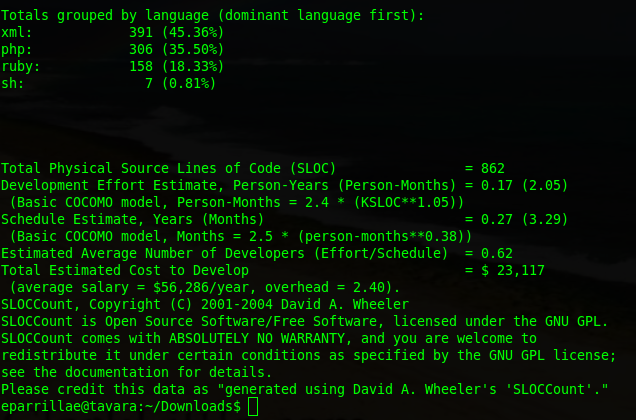
\includegraphics[width=15cm, keepaspectratio]{img/senchasloccount.png}
    \caption{\textit{Sencha Touch Programming Languages}}
    \label{figure:jquerylanguages}
 \end{figure}

We see that most of the code is done using PHP and XML, but also there is some code in Ruby and shell scripts, which means that for implementing mobile apps using this framework requires knowledge in those languages. This is good for me as I have used them extensively in the past.

In the \textbf{Support} category, we can clearly see that the mailing lists work very well and also it is possible to have professional support (see professional support \cite{sencha support}) which is a missing capability in jQuery Mobile. So for this category Sencha is better than jQuery.

Regarding \textbf{Documentation} category, I have to say that the project is really well-documented. There are lots of books about Sencha Touch and the web site contains all necessary resources for both developers without experience and advanced ones, in this category all scores are high. This applies also for \textbf{Adoption} category, there are many real-world examples of mobile apps developed using Sencha Touch framework.

In the \textbf{Community} category, we see that average volume of messages in the mailing lists in the last six months is high. Unfortunately the number of commits in the last month and the number of contributors in this period cannot be checked, as we said before, there is no public access to Sencha Touch code repository. 

In terms of Longevity, Sencha Touch is considered still a young project but taking into account that it is supported by its parent project Sencha\footnote{http://sencha.com/}, managed by a private company\footnote{http://www.sencha.com/company/}  which has several private partners, I think the future of the project is ensured.

In the \textbf{Professionalism} category, we can see that there is a dedicated conference for Sencha users\cite{sencha Conferences} that promotes the framework among its users  (next Sencha Conference to be held in June 2013\footnote{http://senchacon.com/rockstar-promotion/}).

A big difference is that there is no way to contribute to Sencha Touch in the same way it is done in jQuery, i.e., contacting directly with its community and join them, I consider this another important pitfall. The only information I have found related to developers is in the support pages, see Sencha Devs\cite{sencha Devs}.  

Finally jQuery Mobile is licensed using a dual licensing schema\footnote{http://www.oss-watch.ac.uk/resources/duallicence2}  with a commercial license and an Open Source GPLv3 license\footnote{http://gplv3.fsf.org/}. For the KuDo project I was thinking about using a weak-copyleft/permissive license like MIT\footnote{http://opensource.org/licenses/MIT}, BSD\footnote{http://opensource.org/licenses/BSD-3-Clause}, APL\footnote{https://www.apache.org/licenses/LICENSE-2.0.html} , EPL\footnote{http://www.eclipse.org/legal/epl-v10.html}, etc.. This is because my idea is to integrate several tools within my own development and in some cases GPL does not allow me to do so. 

The table below summarize using a SWOT analysis the advantages and disadvantages of Sencha Touch after the OpenBRR analysis:

\begin{figure}[H]
    \centering
    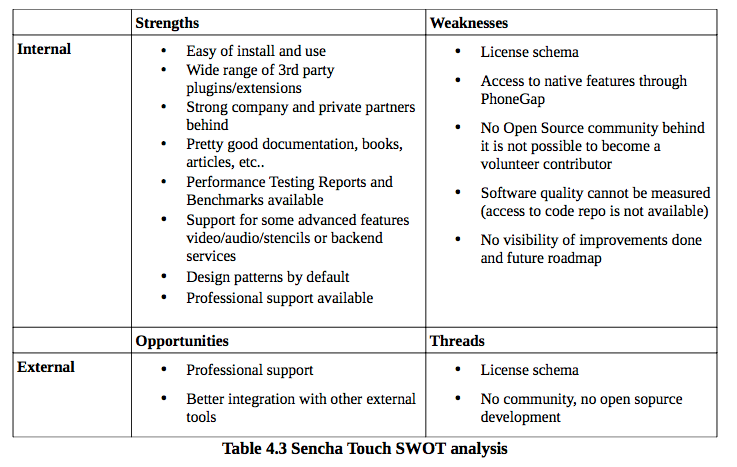
\includegraphics[width=12cm, keepaspectratio]{img/table43.png}
 \end{figure}

%%%%%%%%%%%%%%%%%%%%%%%%%%%%%%%%%%%%%%

\chapter{Conclusions}
\label{chap:conclusions}

In this trade-off study, I have used OpenBRR as Quality Assurance (QA) methodology. I have to say that I believe this methodology covers most of the main aspects of a given project in terms of functionality, usability, scalability, etc.. Also the fact of having templates that automate the calculation of the overall score for each solution is really useful, so I think for me it is a very good way to start evaluating a given solution for my KuDo project.

While evaluating the metrics I saw that there were some analysis aspects that were out of the scope of OpenBRR templates and it was necessary to introduce new metrics to complete the study, specially to provide a "community oriented" point of view.

In the Overview section of this study I have explained the goals of the KuDo project, the idea is to setup a start-up focused in the development of web-based applications for educational purposes that can be easily run in mobile devices such as smartphones, tablets, etc..

During this trade-off I have discovered that jQuery Mobile has the simpler code using a relatively small object model that allows you re-use already existing HTML code, which makes it faster and easier to learn. Sencha has a large object model, which provides more features out of the box (DOM manipulation, CRUD Operations, access to SOAP/REST web services etc...), but takes longer to learn.

There is no established architecture, jQuery Mobile is layout-based and this allows you the freedom to do whatever you want. It is true that it extensively uses Javascript and HTML but for me is a challenge to improve my knowledge in those fields. Also it is easier to integrate with other frameworks, targets more devices than Sencha Touch (Sencha Touch is in a bit of a bind having tied themselves to WebKit) and it is not tied to a particular vendor.

Moreover it is licensed under a MIT weak copyleft license which is perfect for my KuDo project. Clearly Sencha Touch bussiness model is quite different from jQuery Mobile in the case of Sencha there is a clear objective of monetization of their products (closed development process right now and a commercial entity controls it, not an Open Source foundation). For that reason they take care of professional support, implementation of comercial tools for development with Secncha, etc.. But for me this is not relevant as I am an experienced developer and do not need that kind of support. What I am expecting from the selected solution is to have a strong Open Source community behind in which I can also get involved at some point.

As a final conclusion, I would say that if you intend to design business-friendly web apps then probably Sencha is the right option but if your goal is to create a market-friendly apps (like the ones within KuDo project) in a quick time, then you may choose to go with jQuery Mobile.

%%%%%%%%%%%%%%%%%%%%%%%%%%%%%%%%%%%%%%

\chapter{Future Work}
\label{chap:future}

Beginning this year I started working on a new personal project that I called 'KuDo', this is the first time I am going to setup a start-up project from scratch but it has been a long time since I had the idea to do it. 

The first step I took was to define the activity I would like to perform in the start-up  and give it a name, for me it was clear that the new project should be focused in software development and after some "brainstorming" I saw some niche of opportunitties in the educational field and therefore decided to focus the activity in providing lightweight web-based applications for educational purposes that can be easily run in mobile devices such as smartphones, tablets etc... the name "KuDo" was also part of that brainstorming activity :-)

The second step was to look in the market which frameworks were available for mobile apps development, if it was better to go for a native, an hybrid or a web-based solution, and after selecting which approach was better then perform a deep trade-off to be able to take one of these frameworks as baseline solution for my own implementations. This has been the aim of this Master Thesis, during this process I have learnt a lot in terms of web-based technologies, mobile apps and QA metrics.

And now what? Well, as part of the future work on the KuDo project I am planning the following activities:

\begin{itemize}
 \item \textbf{1. Business Model}. One of the requirements I have put on KuDo project is that it has to be  released as an Open Source project, my idea is to review the list of Open Source business models we saw in the MSWL and then take a decision. A dual licensing schema could be interesting, where the "core" of the system is Open Source, released under a GPLv3.0 license and the code is available in one of the most common forges used like GitHub or Launchpad and apart from that there can be commercial licensed extra plugins for the apps and also for support services.
 \item \textbf{2. Training}. Because this is the first time I am setting a start-up I am going to look for some training on this matter, I have found several interesting places to get training and resources like Barcelona Activa\footnote{http://www.barcelonactiva.cat/barcelonactiva/es/agenda.do} , Barcelona Net Activa\footnote{http://www.barcelonanetactiva.com/barcelonanetactiva/en/company-creation/index.jsp} etc...
 \item \textbf{3. Co-working}. Currently I have no space for working at home for that reason I am looking for a coworking\footnote{http://en.wikipedia.org/wiki/Coworking} place that covers the basics that I would need (Internet connection, telephone, proper meeting desk etc...) I have found some interesting places like MeetBCN\footnote{http://www.meetbcn.com/servicios/coworking/} , Comunidad Coworking\footnote{http://www.comunidadcoworking.es/resultatscompra.asp?zona=2}  and Mob Barcelona\footnote{http://www.mob-barcelona.com/} .
\end{itemize}

As a final thougth, now with the crisis which unfortunately is affecting professionally all of us having a long-term job is not guaranteed and I see that it is time to move on and look for new professional opportunities which is exactly what I plan to do with my KuDo project :-)

%%%%%%%%%%%%%%%%%%%%%%%%%%%%%%%%%%%%%%

\chapter{Apendix A: jQuery Mobile "Hello World" Prototype}
\label{Apendix A: jQuery Mobile "Hello World" Prototype}

% pantallazos sobre instalación y proyecto jQuery Mobile

\chapter{Apendix B: Sencha Touch "Hello World" Prototype}
\label{Apendix B: Sencha Touch "Hello World" Prototype}

% pantallazos sobre instalación y proyecto Sencha Touch

%%%%%%%%%%%%%%%%%%%%%%%%%%%%%%%%%%%%%%%%%%%%%%%%%%%%%%%%%%%%%%%%%%%%%
\begin{thebibliography}{25}
\bibliographystyle{alpha} 

\bibitem{OpenBRRWhitepaper}\textbf{OpenBRR: Business Readiness Rating for
Open Source (White paper)}\\
{\footnotesize\url{
http://docencia.etsit.urjc.es/moodle/mod/resource/view.php?id=4343}}

\bibitem{The OpenBRR Corporate Community}\textbf{The OpenBRR Corporate Community}\\
{\footnotesize\url{http://blogs.the451group.com/opensource/2006/04/26/the-openbrr-corporate-community/}}

\bibitem{jquery}\textbf{jQuery Mobile}\\
{\footnotesize\url{http://jquerymobile.com/}}

\bibitem{sencha}\textbf{Sencha Touch}\\
{\footnotesize\url{http://www.sencha.com/products/touch}}

\bibitem{Ohloh}\textbf{Ohloh}\\
{\footnotesize\url{http://www.ohloh.net/}}

\bibitem{ojquery}\textbf{Ohloh jQuery Mobile}\\
{\footnotesize\url{https://www.ohloh.net/p/jquerymobile}}

\bibitem{ojqueryparent}\textbf{Ohloh jQuery}\\
{\footnotesize\url{https://www.ohloh.net/p/jQuery}}

\bibitem{osencha}\textbf{Ohloh Sencha}\\
{\footnotesize\url{https://www.ohloh.net/p/sencha}}

\bibitem{Ohloh Sencha Touch}\textbf{Ohloh Sencha Touch}\\
{\footnotesize\url{https://www.ohloh.net/p?ref=homepage\&q=sencha+touch}}

\bibitem{FLOSSMetrics}\textbf{FLOSSMetrics}\\
{\footnotesize\url{http://flossmetrics.org/}}

\bibitem{FLOSSmole}\textbf{FLOSSmole}\\
{\footnotesize\url{http://flossmole.org/}}

\bibitem{FLOSShub}\textbf{FLOSShub}\\
{\footnotesize\url{http://flosshub.org/}}

\bibitem{FLOSSpapers}\textbf{FLOSSpapers}\\
{\footnotesize\url{http://flosshub.org/biblio}}

\bibitem{linkedin1}\textbf{iPhone, Android, iPad, Tablet, Mobile LinkedIn group}\\
{\footnotesize\url{http://www.linkedin.com/groups/iPhone-Android-iPad-Tablet-Mobile-2013391}}

\bibitem{linkedin2}\textbf{Mobile Software Development LinkedIn group}\\
{\footnotesize\url{http://www.linkedin.com/groups/Mobile-Software-Development-Group-69893}}

\bibitem{linkedin3}\textbf{Developers HTML5, Android, iOS, Blackberry LinkedIn group}\\
{\footnotesize\url{http://www.linkedin.com/groups?home=&gid=54723&trk=anet_ug_hm}}

\bibitem{wikipedia1}\textbf{Wikipedia Web Based Application Framework comparison}\\
{\footnotesize\url{http://en.wikipedia.org/wiki/Multiple_phone_web_based_application_framework}}

\bibitem{wikipedia2}\textbf{Wikipedia Comparison of JavaScript frameworks}\\
{\footnotesize\url{http://en.wikipedia.org/wiki/Comparison_of_JavaScript_frameworks}}

\bibitem{jQuery Mobile Github repo}\textbf{jQuery Mobile Github repo}\\
{\footnotesize\url{https://github.com/jquery/jquery-mobile}}

\bibitem{jQuery Mobile resources}\textbf{jQuery Mobile resources}\\
{\footnotesize\url{http://jquerymobile.com/resources/}}

\bibitem{jQuery Foundation}\textbf{jQuery Foundation}\\
{\footnotesize\url{https://jquery.org/}}

\bibitem{jQuery Roadmap}\textbf{jQuery Roadmap}\\
{\footnotesize\url{https://github.com/jquery/jquery-mobile/wiki/Roadmap}}

\bibitem{jQuery Issues}\textbf{jQuery Issues}\\
{\footnotesize\url{https://github.com/jquery/jquery-mobile/issues}}

\bibitem{jQuery Milestones}\textbf{jQuery Milestones}\\
{\footnotesize\url{https://github.com/jquery/jquery-mobile/issues/milestones}}

\bibitem{jQuery API}\textbf{jQuery API}\\
{\footnotesize\url{http://api.jquerymobile.com/}}

\bibitem{jQuery Themeroller}\textbf{jQuery Themeroller}\\
{\footnotesize\url{http://jquerymobile.com/themeroller/index.php}}

\bibitem{jQuery Demos}\textbf{jQuery Demos}\\
{\footnotesize\url{http://jquerymobile.com/demos}}

\bibitem{jQuery Codiqa}\textbf{jQuery Codiqa}\\
{\footnotesize\url{http://www.codiqa.com/}}

\bibitem{jQuery CDN}\textbf{jQuery CDN}\\
{\footnotesize\url{http://jquerymobile.com/download/}}

\bibitem{sencha Eclipse Plugin}\textbf{sencha Eclipse Plugin}\\
{\footnotesize\url{http://www.sencha.com/blog/sencha-eclipse-plugin-2-0-new-and-noteworthy}}

\bibitem{sencha Architect}\textbf{sencha Architect}\\
{\footnotesize\url{http://www.sencha.com/products/architect}}

\bibitem{sencha performance}\textbf{sencha performance}\\
{\footnotesize\url{http://www.sencha.com/blog/category/html5-developer-scorecard}}

\bibitem{sencha support}\textbf{sencha support}\\
{\footnotesize\url{http://www.sencha.com/support/}}

\bibitem{sencha Learn}\textbf{sencha Learn}\\
{\footnotesize\url{http://www.sencha.com/learn/touch/}}

\bibitem{sencha Demos}\textbf{sencha Demos}\\
{\footnotesize\url{http://www.sencha.com/products/touch/demos/}}

\bibitem{sencha Try}\textbf{sencha Try}\\
{\footnotesize\url{http://try.sencha.com/}}

\bibitem{sencha API}\textbf{sencha API}\\
{\footnotesize\url{http://docs.sencha.com/touch/2.2.1/#!/api}}

\bibitem{sencha MVC}\textbf{sencha MVC}\\
{\footnotesize\url{http://docs.sencha.com/touch/2.2.1/#!/guide/apps_intro}}

\bibitem{sencha Download}\textbf{sencha Download}\\
{\footnotesize\url{http://www.sencha.com/products/touch/download/}}

\bibitem{sencha License}\textbf{sencha License}\\
{\footnotesize\url{http://www.sencha.com/products/touch/license/}}

\bibitem{sencha Conferences}\textbf{sencha Conferences}\\
{\footnotesize\url{http://senchacon.com/}}

\bibitem{sencha Apps}\textbf{sencha Apps}\\
{\footnotesize\url{http://www.sencha.com/apps/}}

\bibitem{sencha Devs}\textbf{sencha Devs}\\
{\footnotesize\url{http://www.senchadevs.com/}}

\bibitem{sencha vs jquery 1}\textbf{sencha vs jquery 1}\\
{\footnotesize\url{http://www.classicinformatics.com/JQuery-Mobile-vs-Sencha-Touch/}}

\bibitem{sencha vs jquery 2}\textbf{sencha vs jquery 2}\\
{\footnotesize\url{http://www.classicinformatics.com/JQuery-Mobile-vs-Sencha-Touch/}}

\bibitem{sencha vs jquery 3}\textbf{sencha vs jquery 3}\\
{\footnotesize\url{http://www.quora.com/Which-is-better-jQuery-Mobile-or-Sencha-Touch}}


\end{thebibliography}
\end{document}
